\documentclass[11pt]{article}
\usepackage{geometry,marginnote} % Pour passer au format A4
\geometry{hmargin=1cm, vmargin=1cm} % 

% Page et encodage
\usepackage[T1]{fontenc} % Use 8-bit encoding that has 256 glyphs
\usepackage[english,french]{babel} % Français et anglais
\usepackage[utf8]{inputenc} 

\usepackage{lmodern,numprint}
\setlength\parindent{0pt}

% Graphiques
\usepackage{graphicx,float,grffile,units}
\usepackage{tikz,pst-eucl,pst-plot,pstricks,pst-node,pstricks-add,pst-fun,pgfplots} 

% Maths et divers
\usepackage{amsmath,amsfonts,amssymb,amsthm,verbatim}
\usepackage{multicol,enumitem,url,eurosym,gensymb,tabularx}

\DeclareUnicodeCharacter{20AC}{\euro}



% Sections
\usepackage{sectsty} % Allows customizing section commands
\allsectionsfont{\centering \normalfont\scshape}

% Tête et pied de page
\usepackage{fancyhdr} \pagestyle{fancyplain} \fancyhead{} \fancyfoot{}

\renewcommand{\headrulewidth}{0pt} % Remove header underlines
\renewcommand{\footrulewidth}{0pt} % Remove footer underlines

\newcommand{\horrule}[1]{\rule{\linewidth}{#1}} % Create horizontal rule command with 1 argument of height

\newcommand{\Pointilles}[1][3]{%
  \multido{}{#1}{\makebox[\linewidth]{\dotfill}\\[\parskip]
}}

\newtheorem{Definition}{Définition}

\usepackage{siunitx}
\sisetup{
    detect-all,
    output-decimal-marker={,},
    group-minimum-digits = 3,
    group-separator={~},
    number-unit-separator={~},
    inter-unit-product={~}
}

\setlength{\columnseprule}{1pt}

\begin{document}

\textbf{Nom, Prénom :} \hspace{8cm} \textbf{Classe :} \hspace{3cm} \textbf{Date :}\\

\begin{center}
  \textit{Il faut apprendre, non pas pour l'amour de la connaissance, mais pour se défendre contre le mépris dans lequel le monde tient les ignorants.}  - \textbf{Charlie Chaplin}
\end{center}

\begin{multicols}{2}
  \subsection*{ex1 - Le compas dans l'œil}

  \textbf{Placer un point $I_1$ milieu de $[A_1 B_1]$ et $I_2$ milieu de $[A_2 B_2]$.}
  \begin{figure}[H]
        \centering
        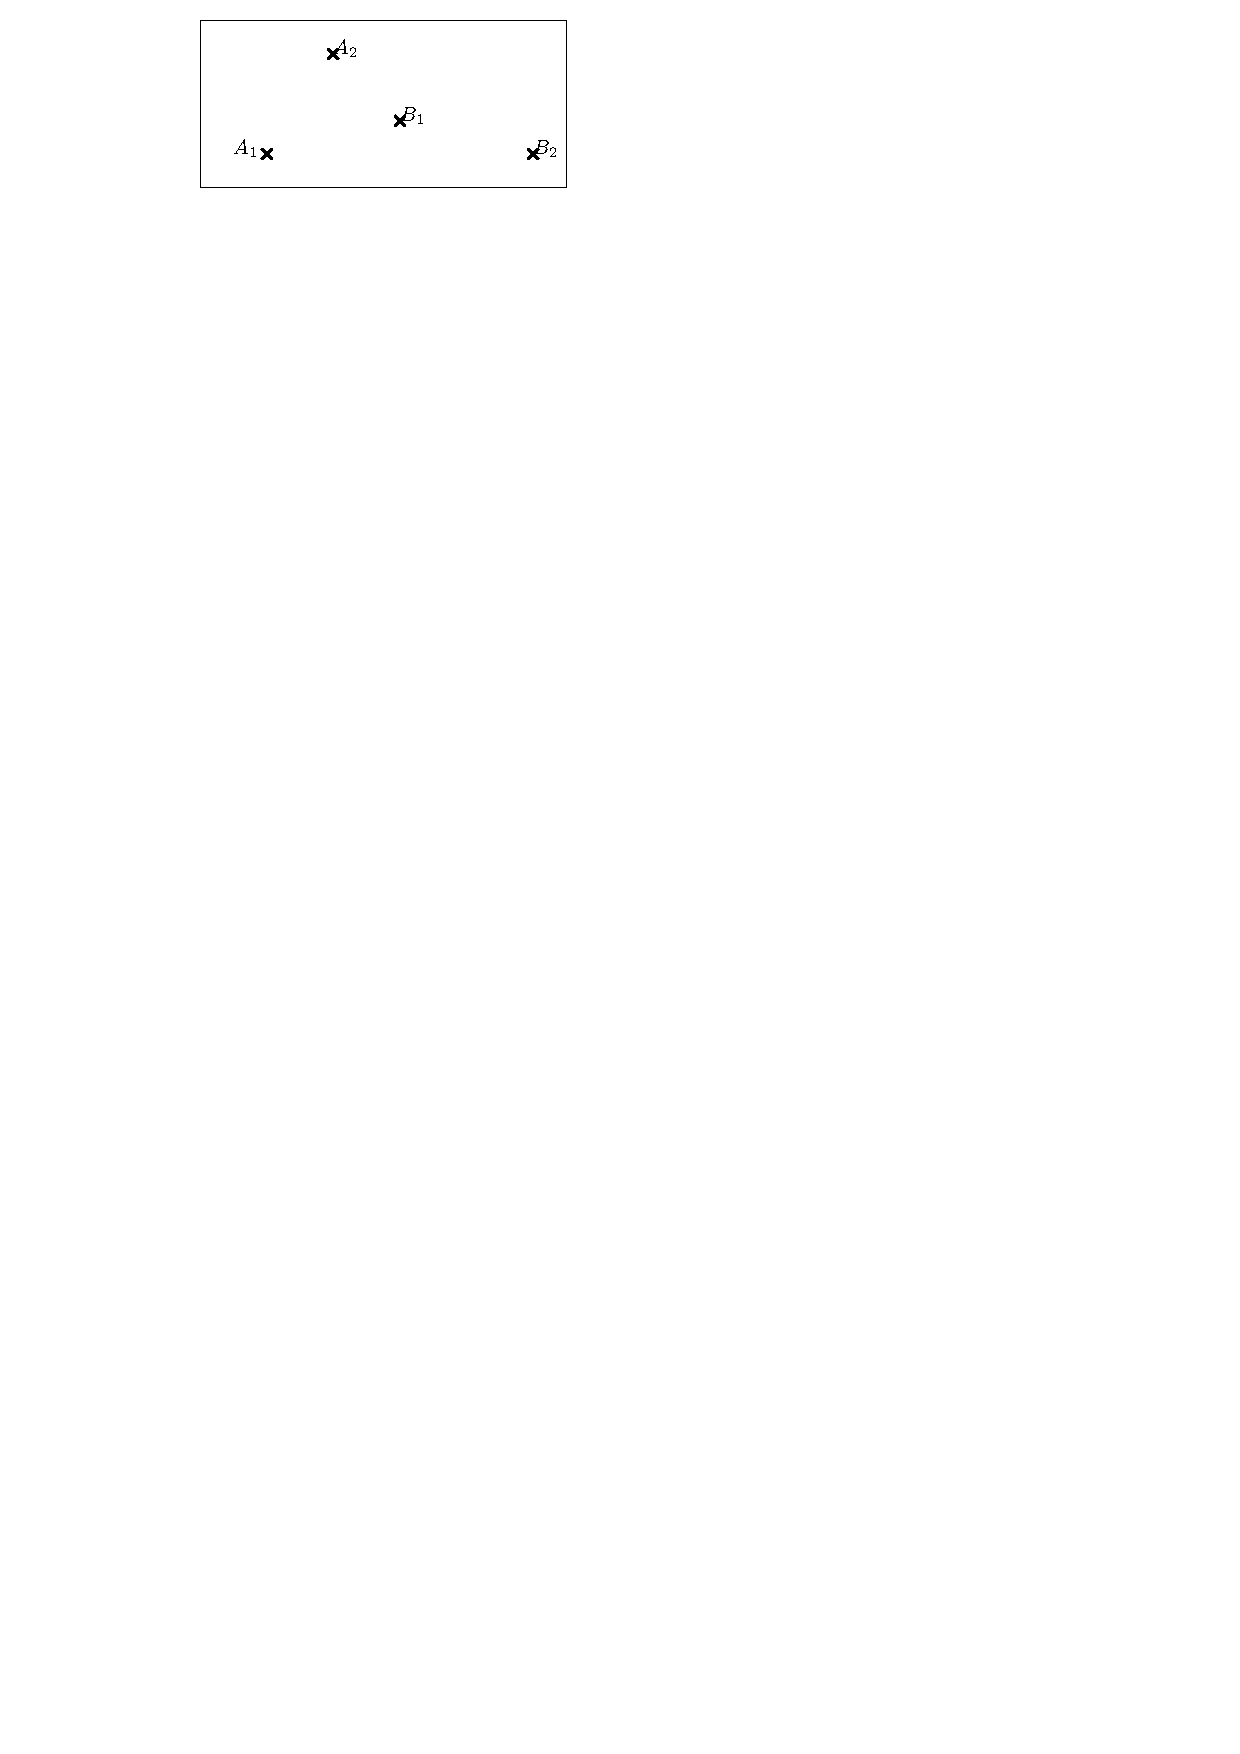
\includegraphics[width=0.8\linewidth]{5x2-symetrie-centrale/5x2-ie-ex1-1.pdf}
  \end{figure}
  \columnbreak

  \textbf{Tracer les droites $(d_1)$ et $(d_2)$ passant par $A_1$ et $A_2$ et parallèles à $(d)$.}
  \begin{figure}[H]
        \centering
        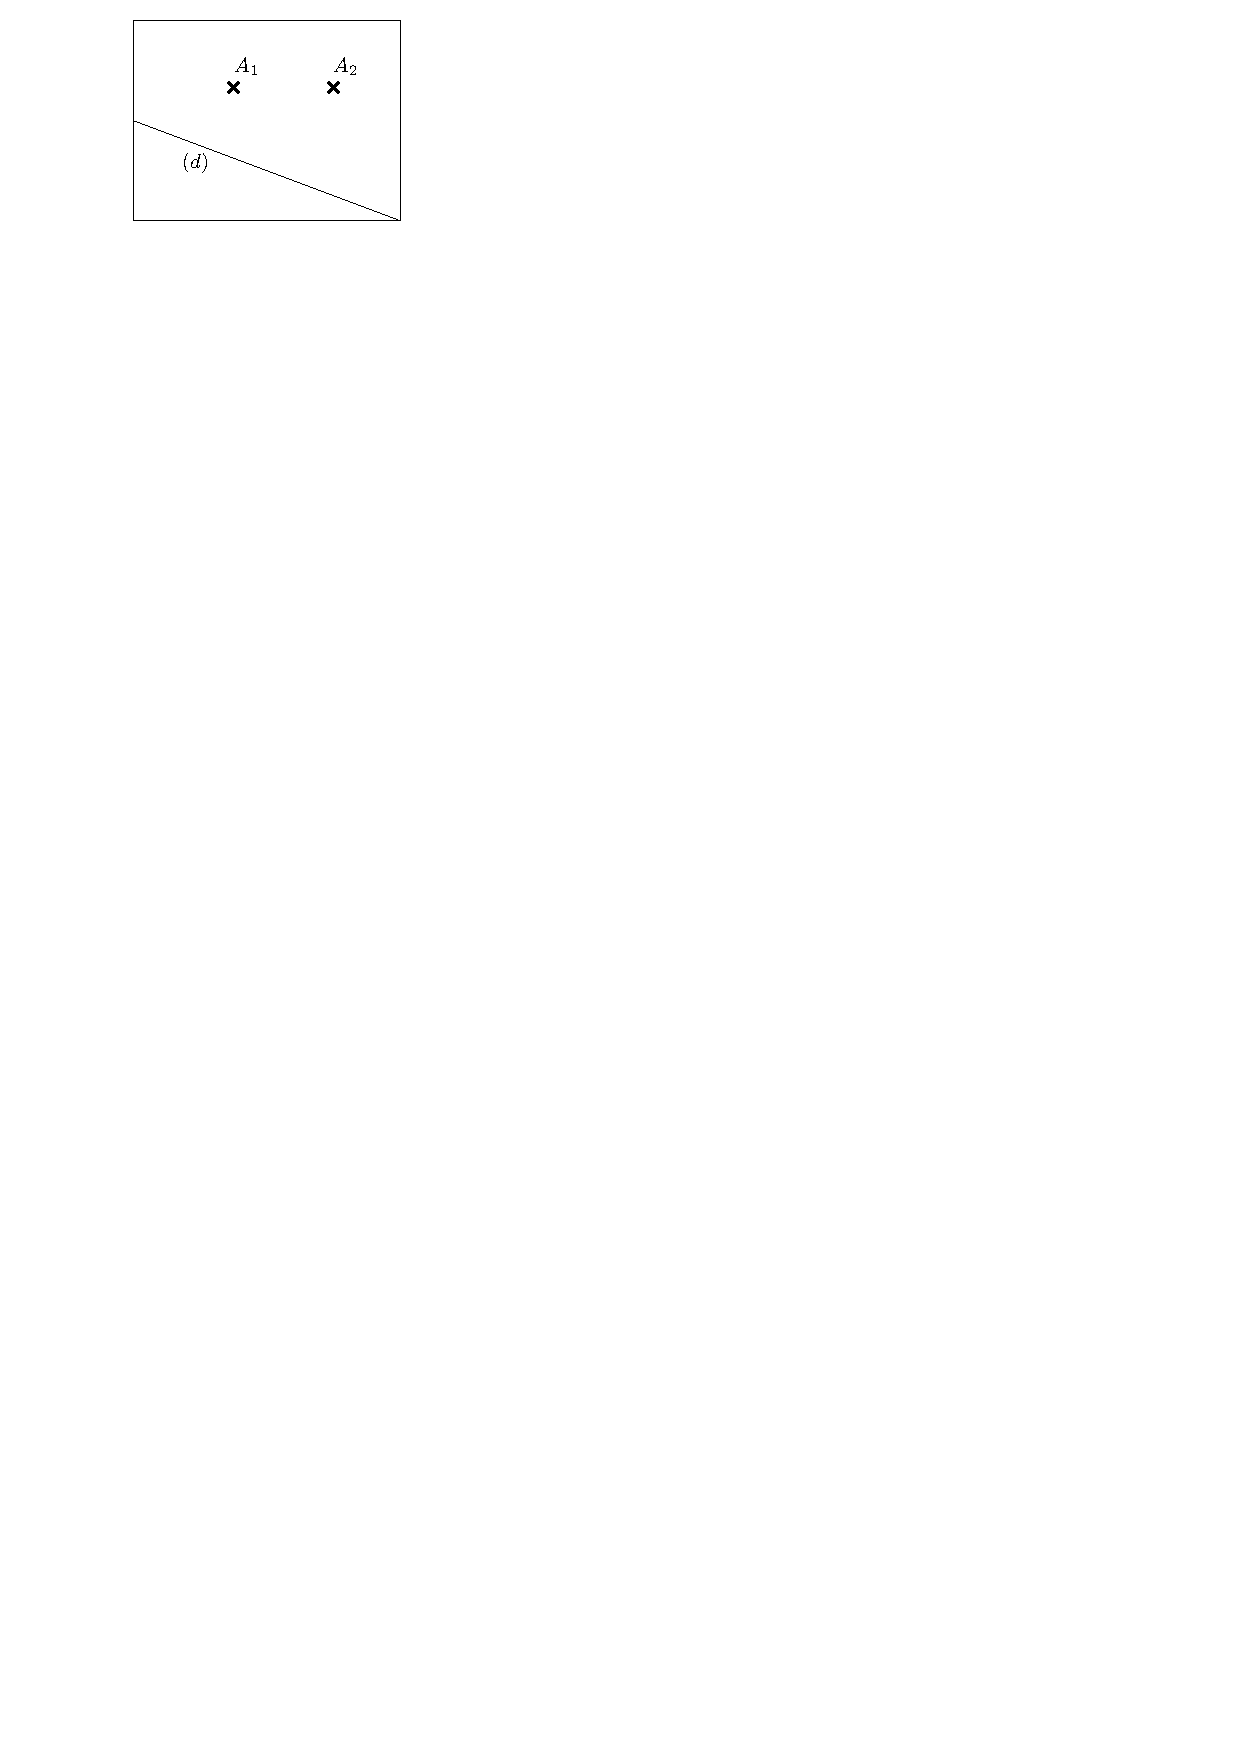
\includegraphics[width=0.8\linewidth]{5x2-symetrie-centrale/5x2-ie-ex1-2.pdf}
  \end{figure}
\end{multicols}

\subsection*{ex2 - À l'aide du quadrillage}

\begin{multicols}{2}

  \textbf{Placer un point $I_1$ milieu de $[A_1 B_1]$ et $I_2$ milieu de $[A_2 B_2]$.}
  \begin{figure}[H]
        \centering
        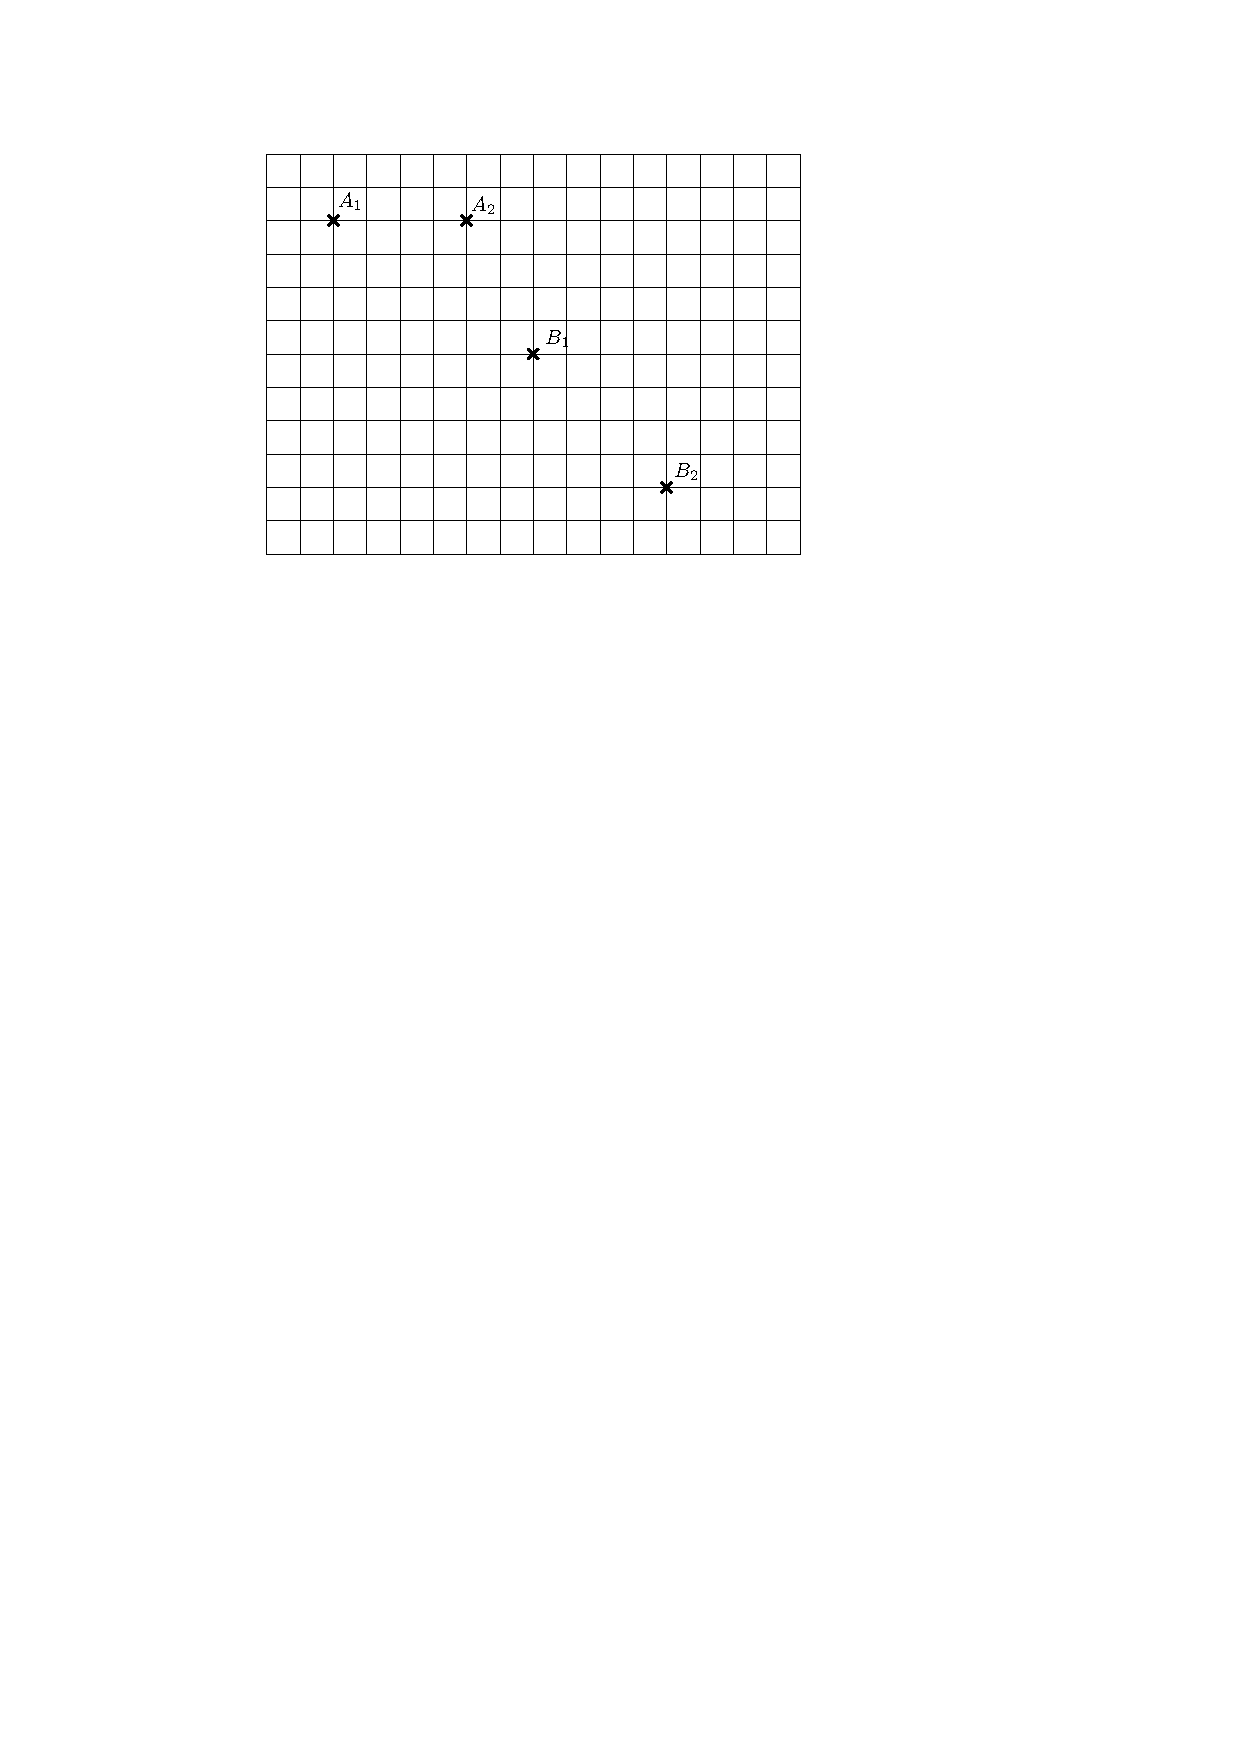
\includegraphics[width=0.8\linewidth]{5x2-symetrie-centrale/5x2-ie-ex2-1.pdf}
  \end{figure}
  \columnbreak

  \textbf{Tracer les droites $(d_1)$, $(d_2)$ et $(d_3)$ passant par $A_1$, $A_2$ et $A_3$ et parallèles à $(d)$.}
  \begin{figure}[H]
        \centering
        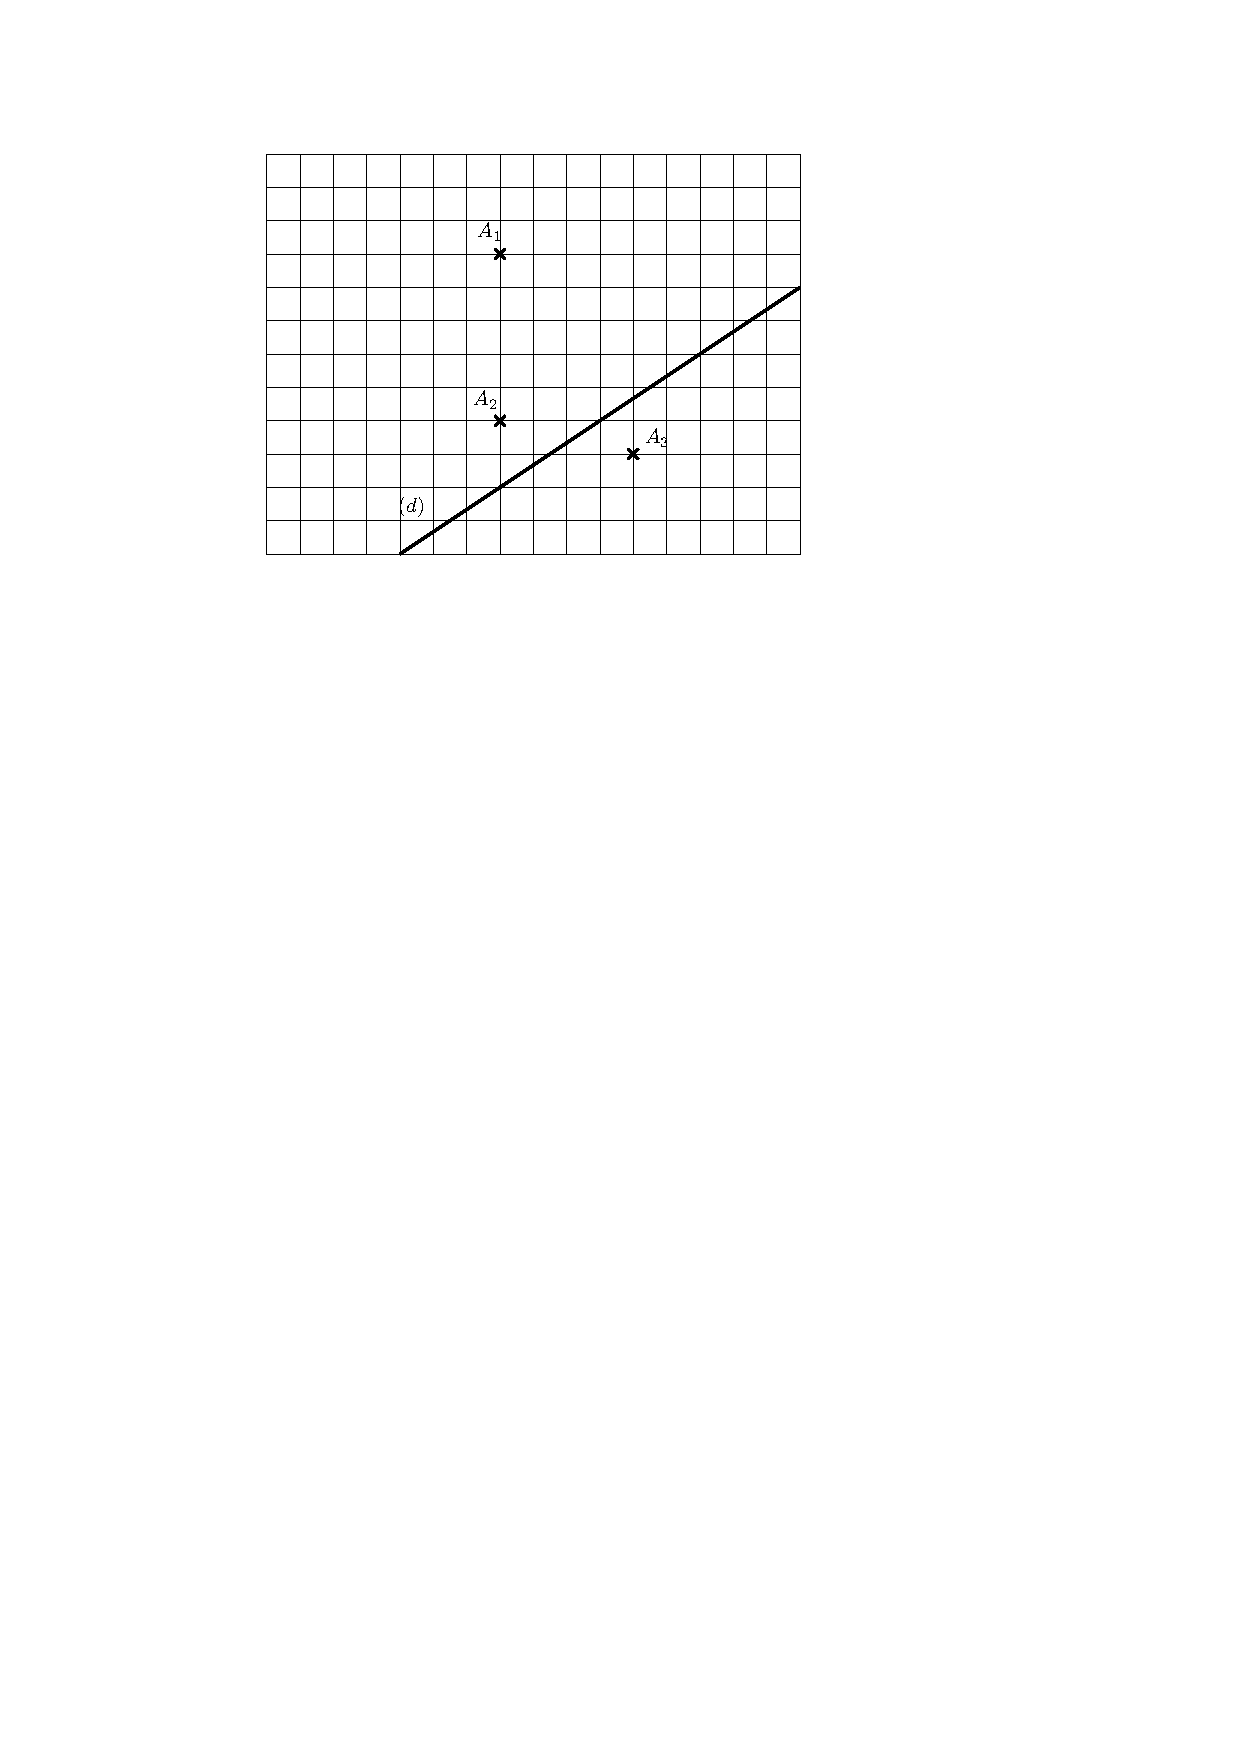
\includegraphics[width=0.8\linewidth]{5x2-symetrie-centrale/5x2-ie-ex2-2.pdf}
  \end{figure}
\end{multicols}

\subsection*{ex3 - Apprendre ses définitions} 

\textbf{Définir un cercle : } \dotfill \newline
\Pointilles[2]

\textbf{Définir une symétrie centrale : }\dotfill \newline
\Pointilles[2]


\textbf{Donner la propriété d'une symétrie centrale : }\dotfill \newline
\Pointilles[2]


\subsection*{ex4 - Symétrie centrale - Quadrillage et feuille blanche}

\textbf{Tracer le symétrique des points A, B et C par rapport à 0.}

\begin{multicols}{2}

  \begin{figure}[H]
        \centering
        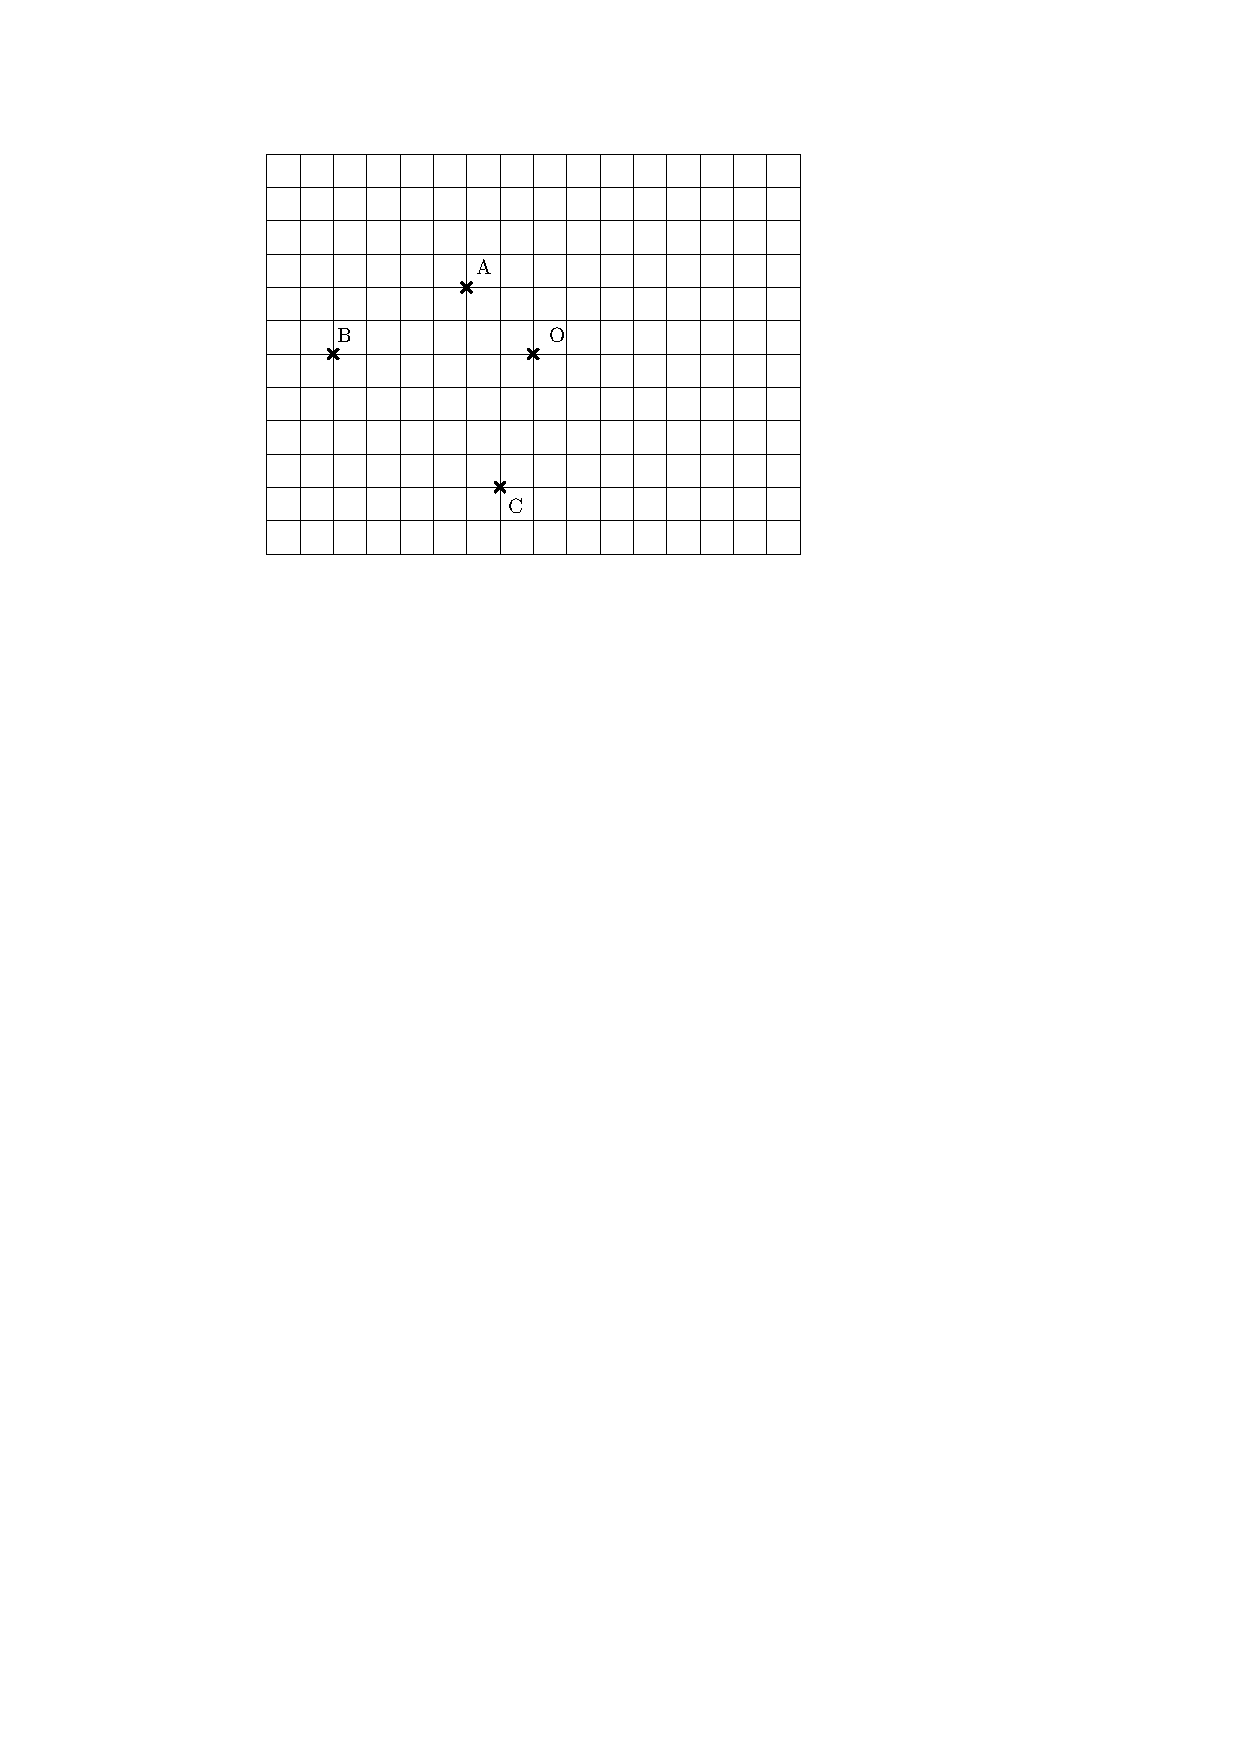
\includegraphics[width=0.9\linewidth]{5x2-symetrie-centrale/5x2-ie-ex4-1.pdf}
  \end{figure}

  \begin{figure}[H]
        \centering
        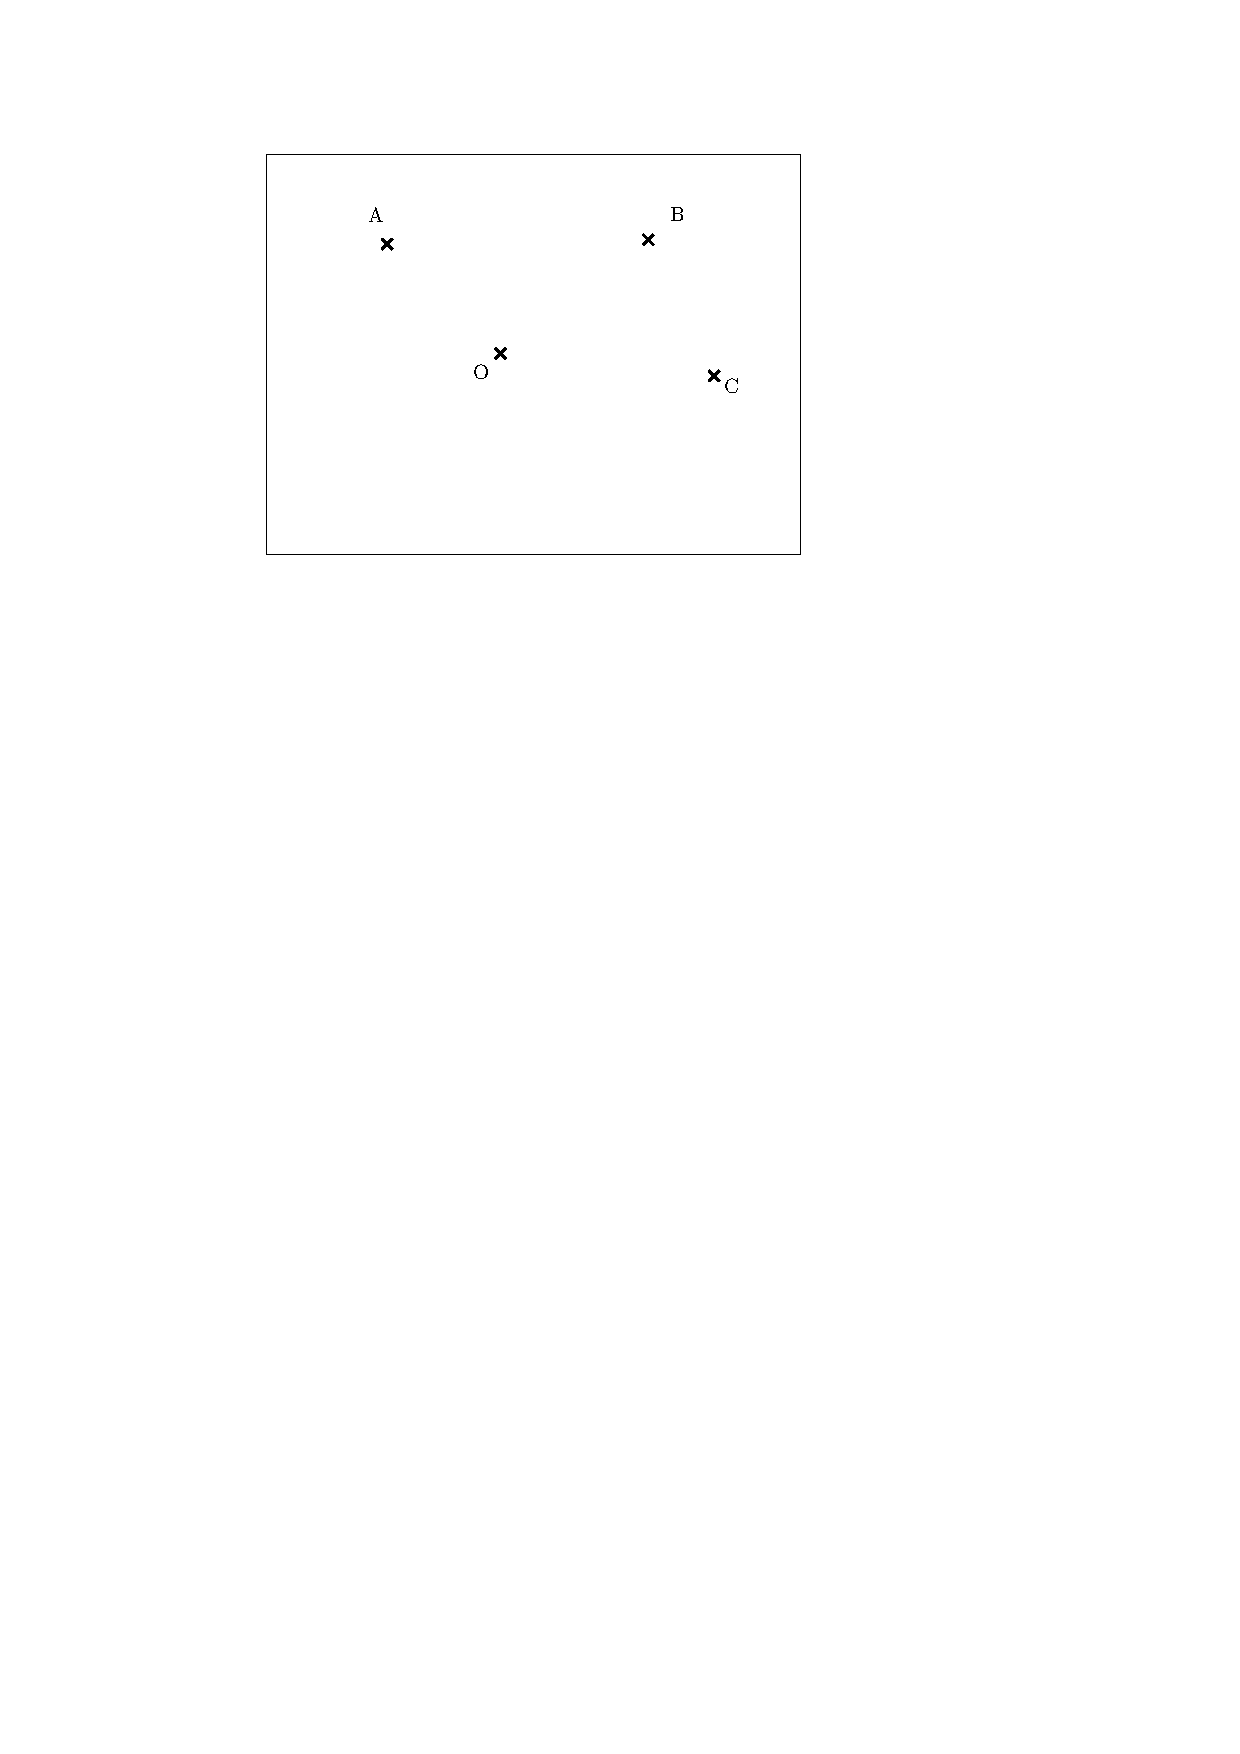
\includegraphics[width=0.9\linewidth]{5x2-symetrie-centrale/5x2-ie-ex5-1.pdf}
  \end{figure}

\end{multicols}

\textbf{Tracer le symétrique du triangle par rapport à 0.}

\begin{multicols}{2}

  \begin{figure}[H]
        \centering
        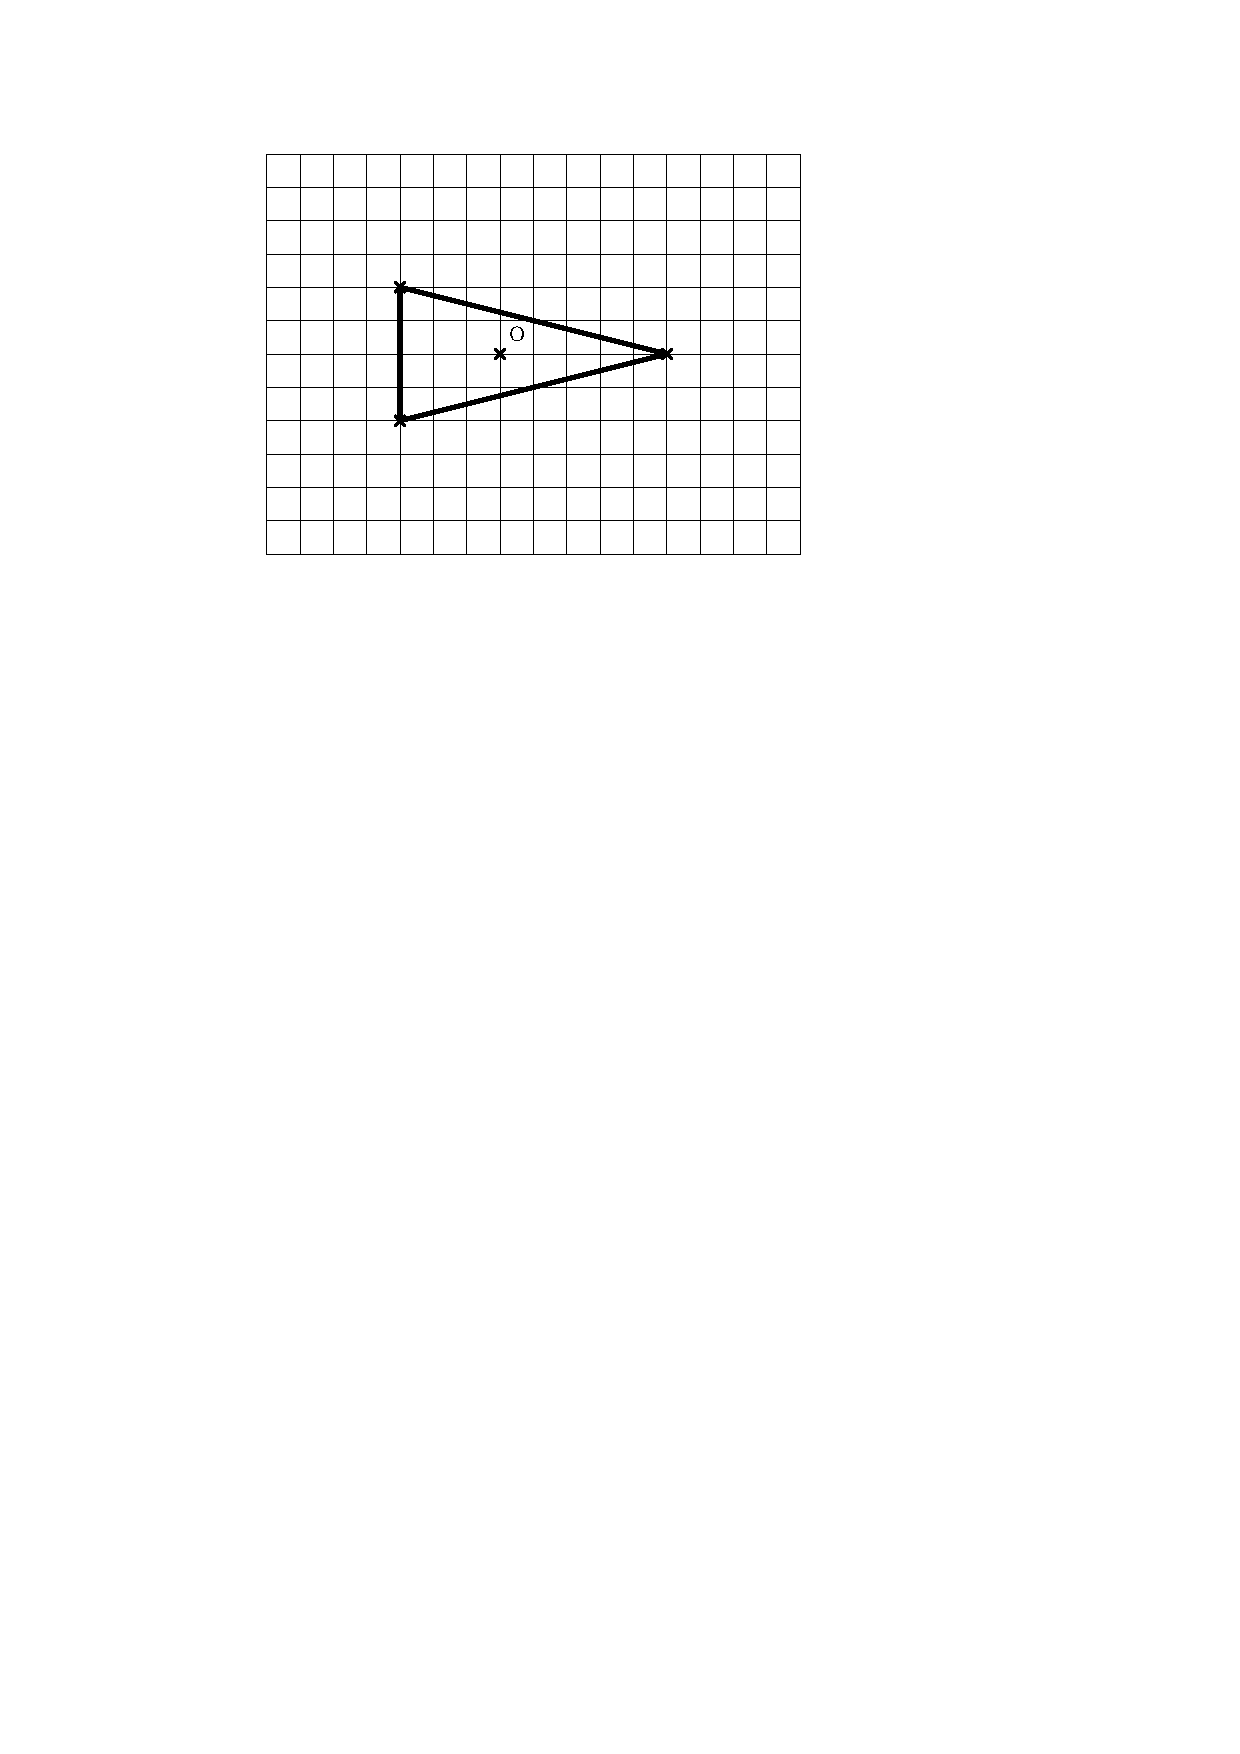
\includegraphics[width=0.9\linewidth]{5x2-symetrie-centrale/5x2-ie-ex4-2.pdf}
  \end{figure}

  \begin{figure}[H]
        \centering
        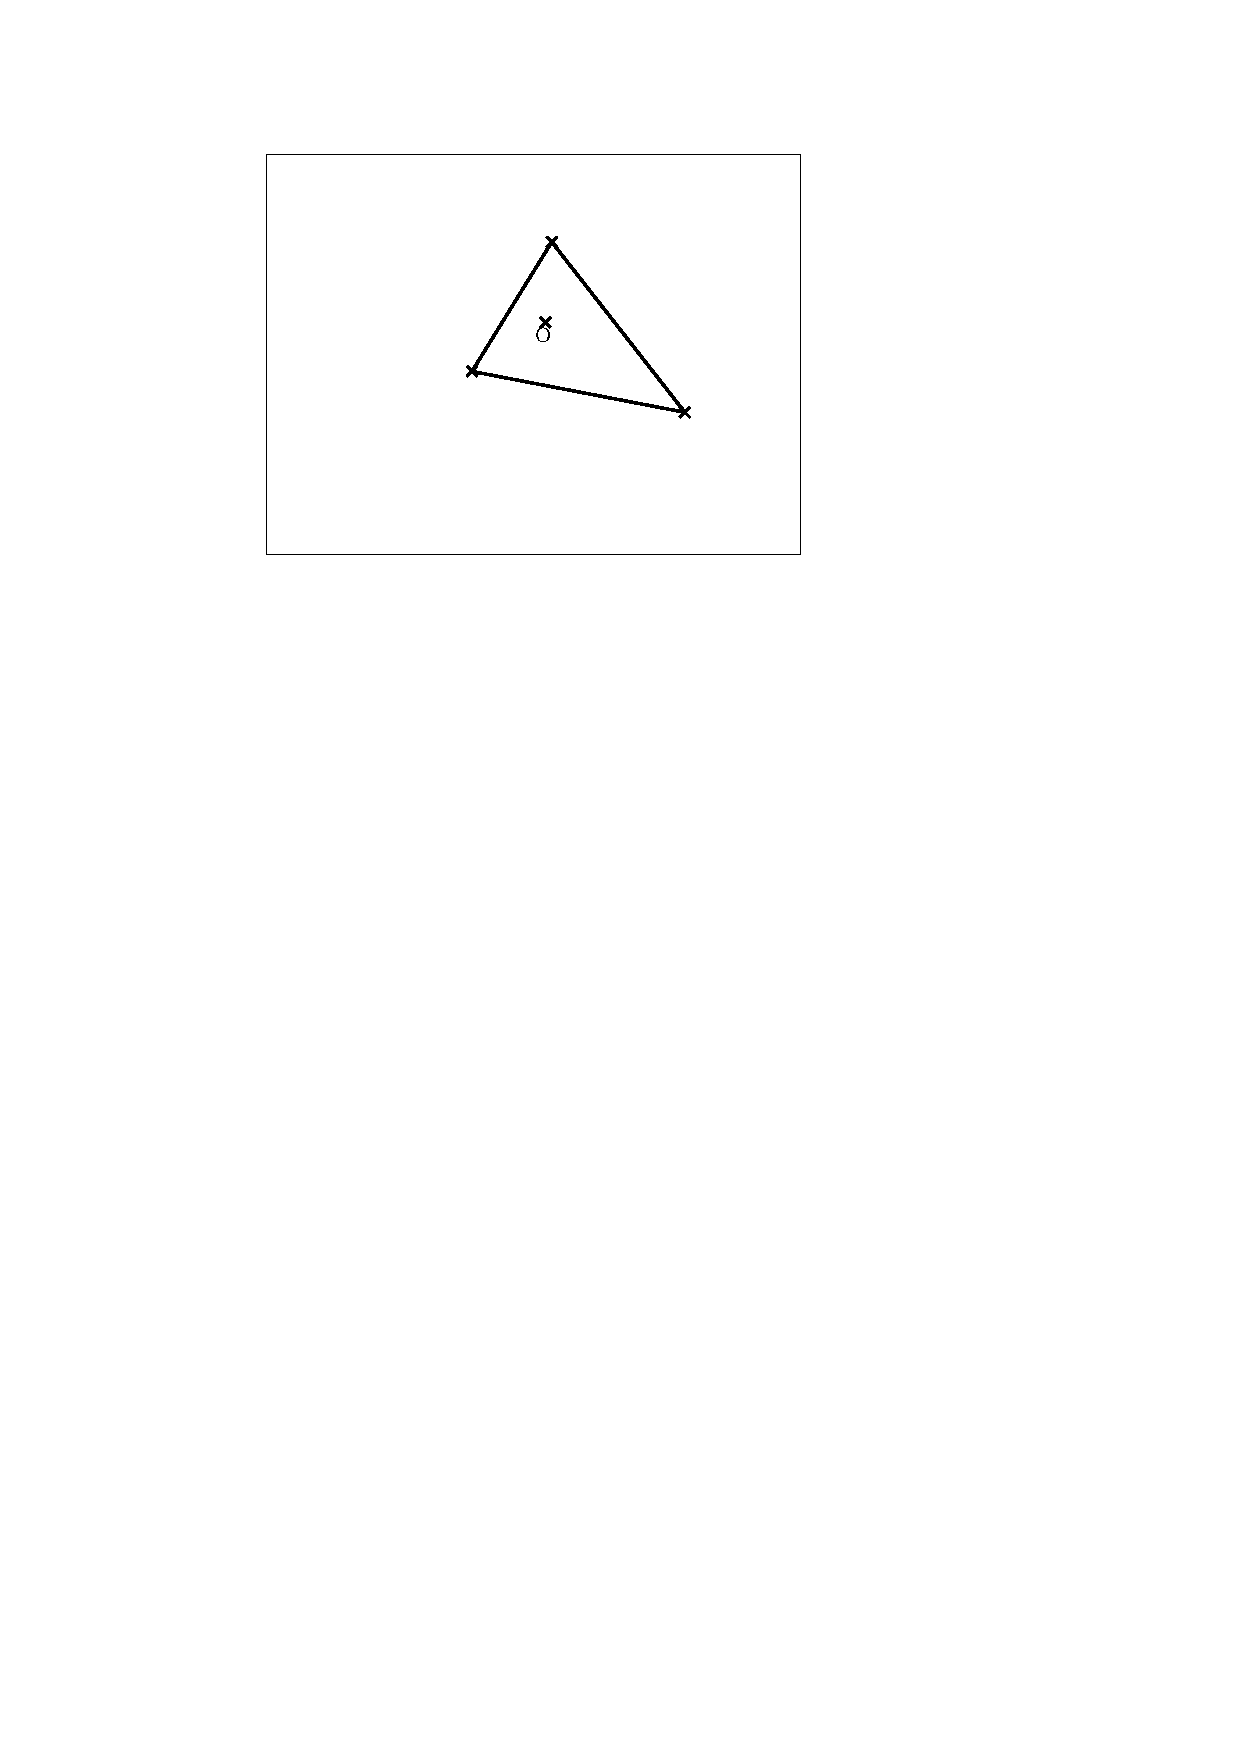
\includegraphics[width=0.9\linewidth]{5x2-symetrie-centrale/5x2-ie-ex5-2.pdf}
  \end{figure}

\end{multicols}

\textbf{Tracer le symétrique de la figure par rapport à 0.}

\begin{multicols}{2}

  \begin{figure}[H]
        \centering
        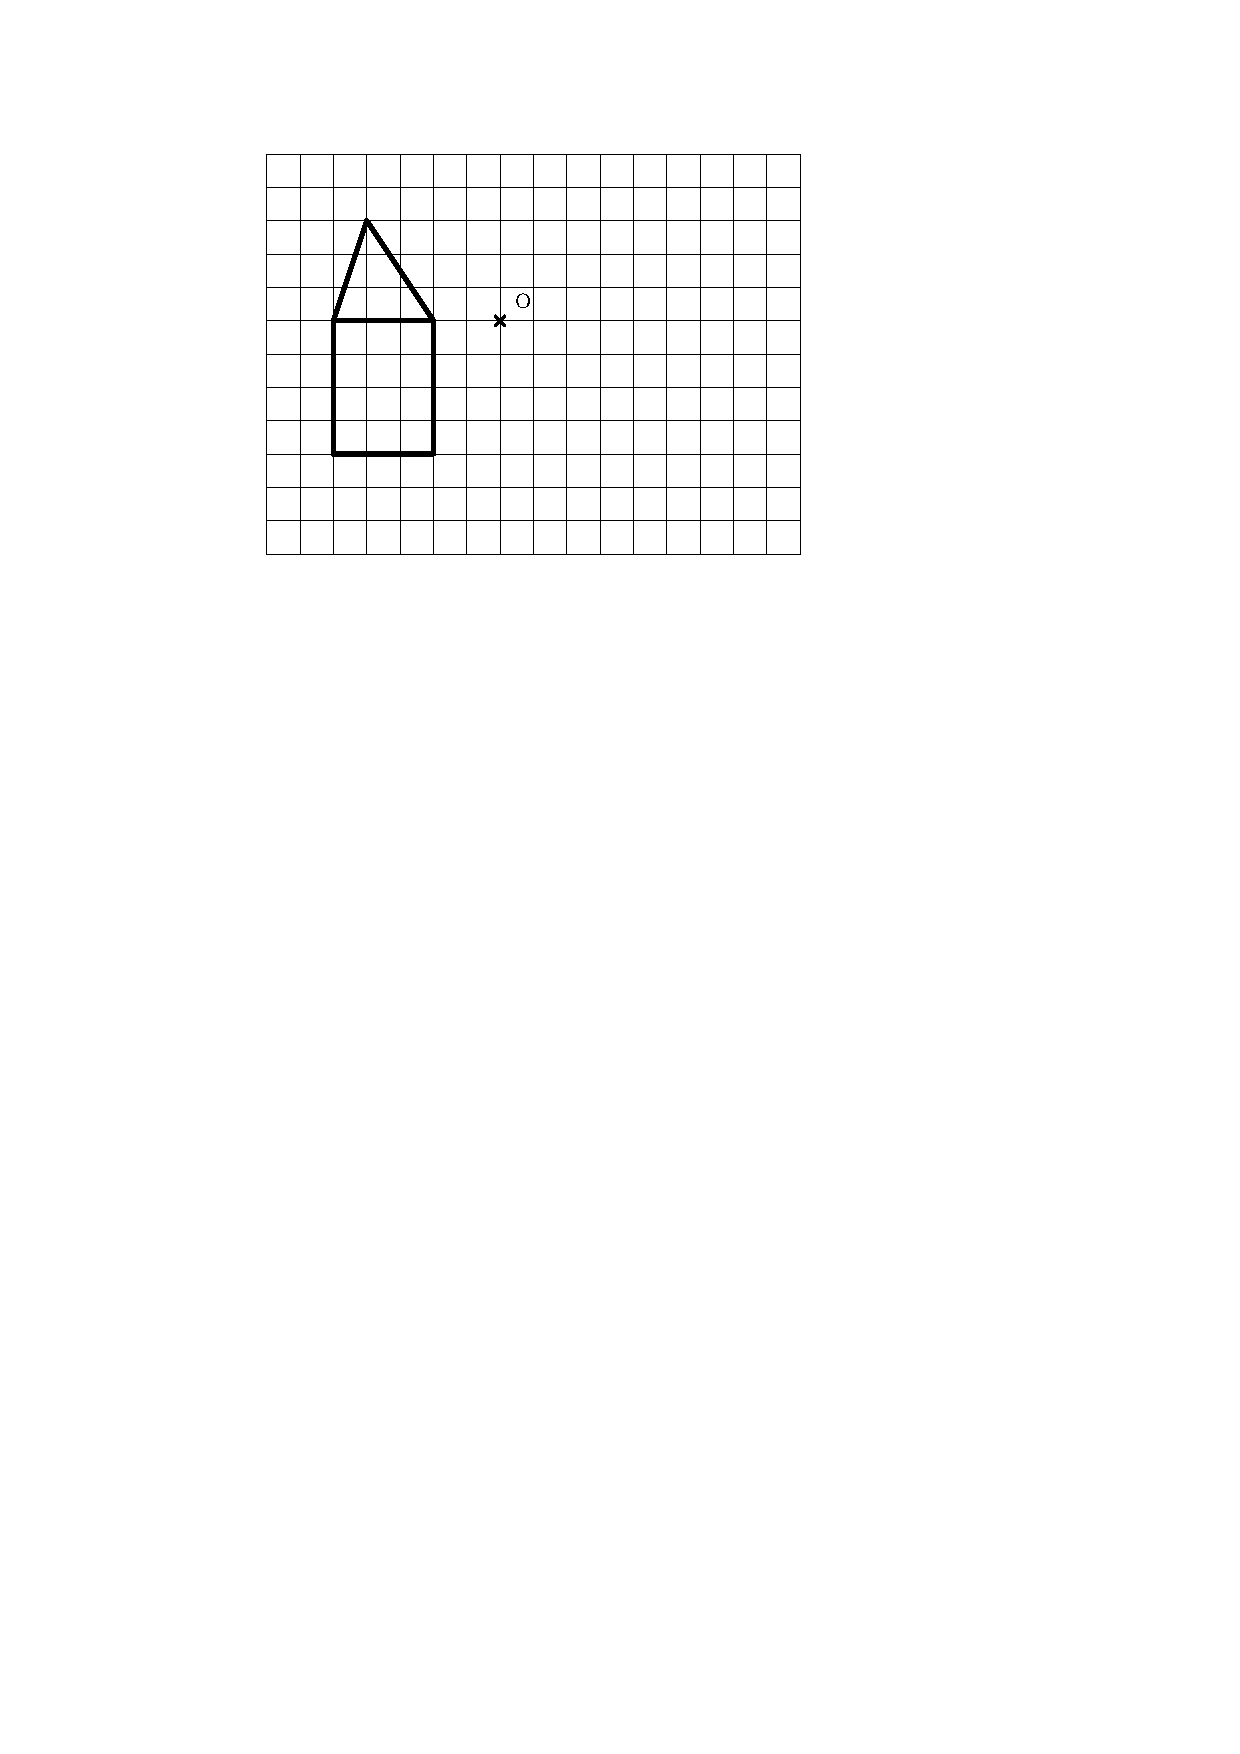
\includegraphics[width=0.9\linewidth]{5x2-symetrie-centrale/5x2-ie-ex4-3.pdf}
  \end{figure}

  \begin{figure}[H]
        \centering
        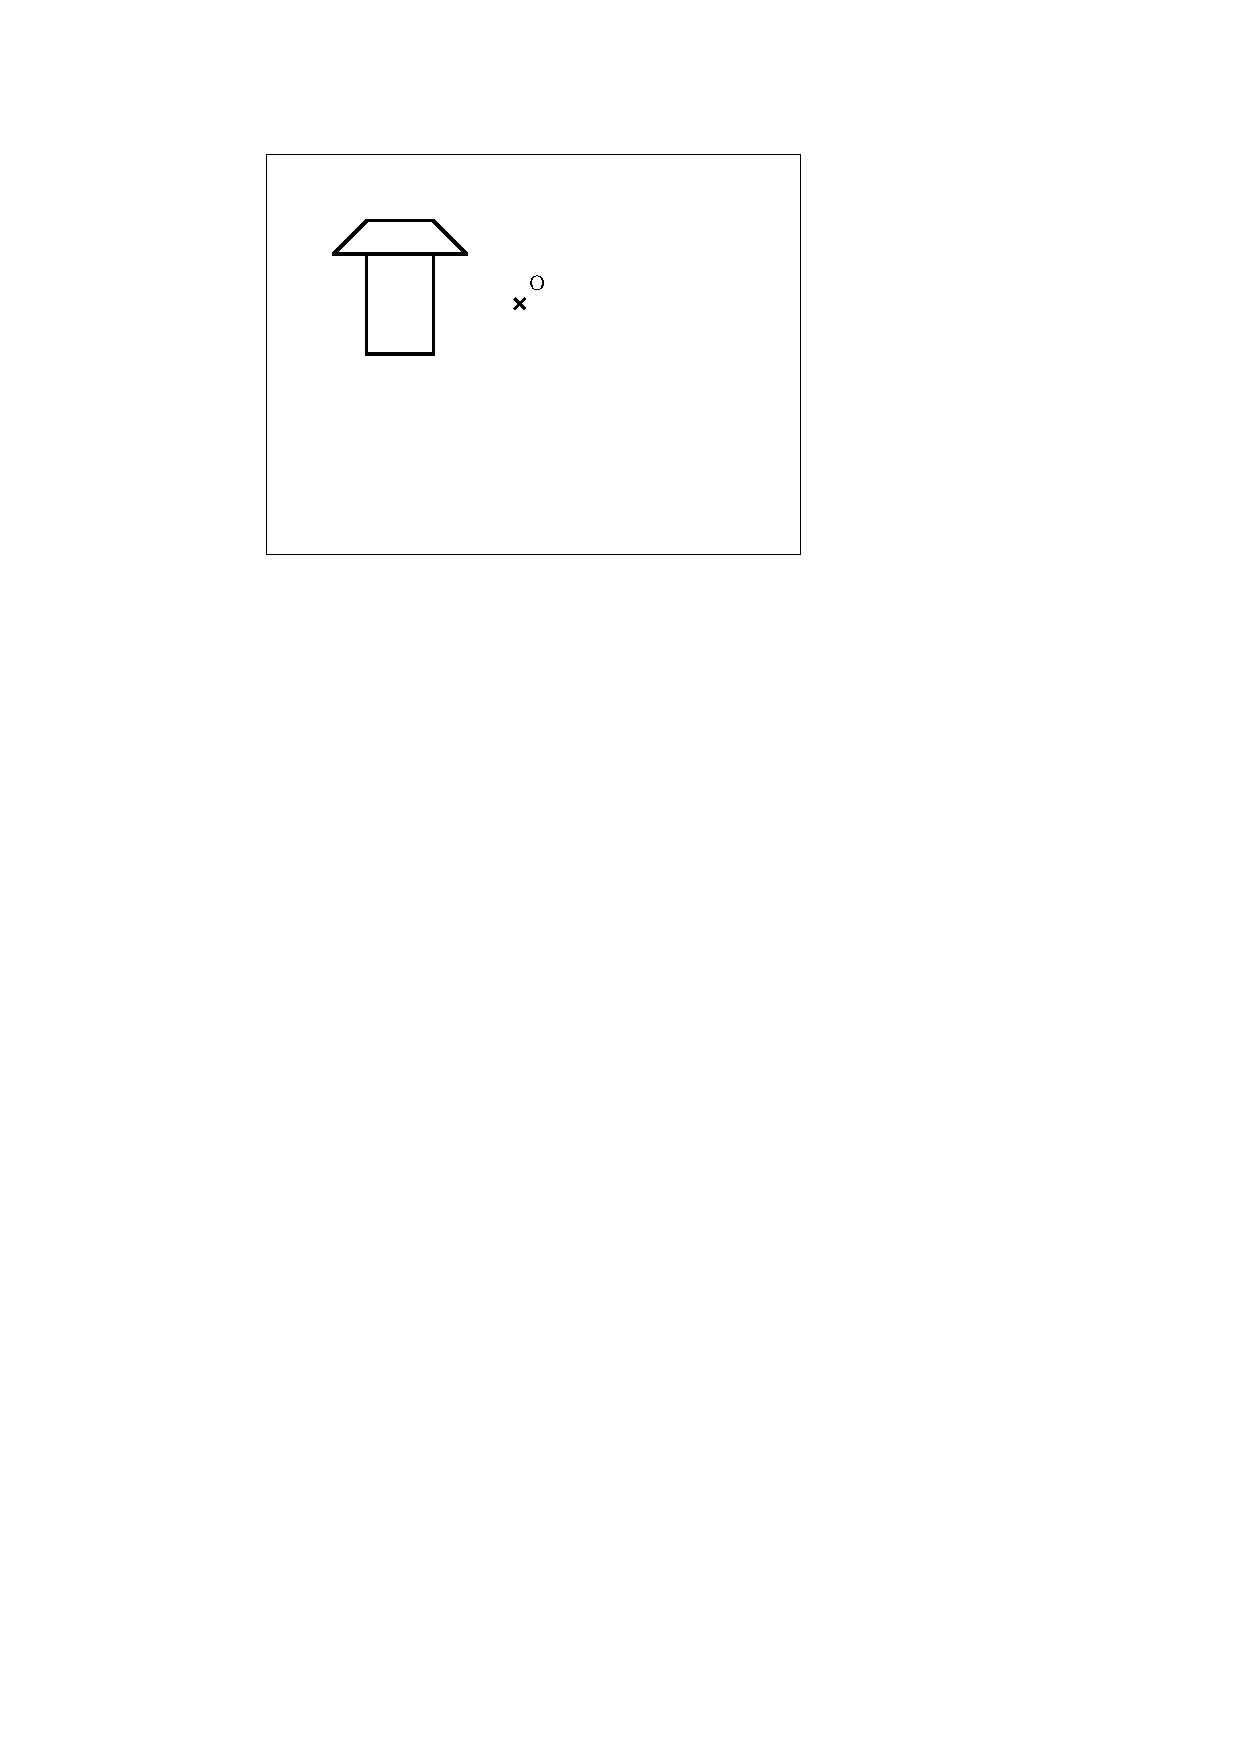
\includegraphics[width=0.9\linewidth]{5x2-symetrie-centrale/5x2-ie-ex5-3.pdf}
  \end{figure}

\end{multicols}

\end{document}